
\section{Four pipes and a span}
\label{Sec:fourpipes}

An example is constructed with five ``rooms'' connected by \zobj{zlinks}.
Four of these room \zobj{zboxen} are designated \emph{Pipe} type containment,
while one is \emph{Span} type. ``Balls'' will be send on \zobj{zpaths} which
traverse the rooms and end in a \zobj{zbox} of type \emph{Sink}.

\begin{figure}[ht]
  \centering
  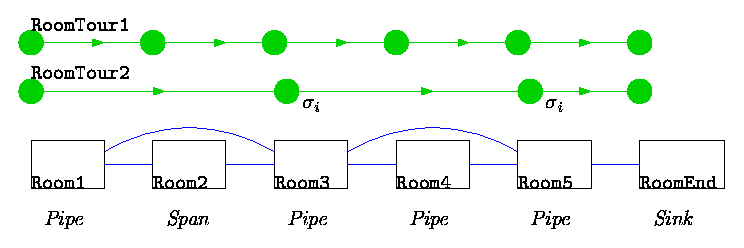
\includegraphics[angle=0,width=12cm]{50_figs/_FiveRooms.eps}
  \caption{Five rooms (black), of \emph{Pipe} and \emph{Span} types: \zobj{zlinks} (blue) allow the two \zobj{zpaths} (green).
    The {\tt RoomTour2} \zobj{zpath} enters {\tt Room3} and {\tt Room5} at non-zero initial position.}
  \label{fiverooms}
\end{figure}


The full zsyntax input is listed below. First global parameters in the \zobj{zsystem} are defined:
\begin{lstlisting}[mathescape]
[zsystem PipeTest T_0 = 0  t_0 = 00:00  t_1 = 12:30  $\Delta$t = 30  R=S ]
\end{lstlisting}
The types of rooms are specified:
\begin{lstlisting}[mathescape]
[ztype A=piperoom n=1 m=Pipe C={Ball 1} L=90 ]
[ztype A=piperoomslow n=1 m=Pipe C={Ball 1} L=90 V=3.1 ]
[ztype A=spanroom n=1 m=Span C={Ball 1} L=90 V=3.1 ]
[ztype A=exitsink n=1 m=Sink C={Ball 1}]
[ztype A=Ball n=1 l=20 v=5 R=SCPd]
\end{lstlisting}
Balls will be inserted into the system; for this a prototype \zobj{zbox} is required:
\begin{lstlisting}[mathescape]
[zbox BallProto A=Ball n=1 $\pi$=1 ]
[zsource BallSource m=One o=Teleport $\phi$=<BallProto>]
\end{lstlisting}
Five rooms can be represented by \zobj{zboxen} and connected with \zobj{zlinks}:
\begin{lstlisting}[mathescape]
[zbox Room1 A=piperoom n=1 ]
[zlink $\mu$=<Room1> $\nu$=<Room2> A={Ball . 1}]
[zlink $\mu$=<Room1> $\nu$=<Room3> A={Ball . 1}] # zlink also from 1-3.
[zbox Room2 A=spanroom n=1 ]
[zlink $\mu$=<Room2> $\nu$=<Room3> A={Ball . 1}]
[zbox Room3 A=piperoom n=1 ]
[zlink $\mu$=<Room3> $\nu$=<Room4> A={Ball . 1}]
[zlink $\mu$=<Room3> $\nu$=<Room5> A={Ball . 1}] # zlink also from 3-5.
[zbox Room4 A=piperoomslow n=1 ]
[zlink $\mu$=<Room4> $\nu$=<Room5> A={Ball . 1}]
[zbox Room5 A=piperoom n=1 ]
[zlink $\mu$=<Room5> $\nu$=<RoomEnd> A={Ball . 1}]
[zbox RoomEnd A=exitsink n=1 ]
\end{lstlisting}
One \zobj{zpath} visits all rooms in order; another visits the same rooms, but
shows the use of explicit entry and exit points:
\begin{lstlisting}[mathescape]
[zpath RoomTour1 A=Ball n=1 m=Open
 $\Lambda$={  # '$\Lambda$' is a list of zstops.
     [zstop $\phi$=<Room1>]
     [zstop $\phi$=<Room2>]
     [zstop $\phi$=<Room3>]
     [zstop $\phi$=<Room4>]
     [zstop $\phi$=<Room5>]
     [zstop $\phi$=<RoomEnd>]
 } ]
[zpath RoomTour1a A=Ball n=1 m=Open
 $\Lambda$={  # '$\Lambda$' is a list of zstops.
     [zstop $\phi$=<Room1>]
     [zstop $\phi$=<Room2> $\sigma$_i=0.1 $\sigma$_f=0.9 ] # specific entry and exit points
     [zstop $\phi$=<Room3> $\sigma$_i=0.05 $\sigma$_f=0.9 ]
     [zstop $\phi$=<Room4> $\sigma$_i=0.05] 
     [zstop $\phi$=<Room5>]
     [zstop $\phi$=<RoomEnd>]
 } ]
\end{lstlisting}
Another \zobj{zpath} skips rooms 2 and 4; this is possible due to the \zobj{zlink} configuration:
\begin{lstlisting}[mathescape]
[zpath RoomTour2 A=Ball n=1 m=Open $\Lambda$={ [zstop $\phi$=<Room1>] [zstop $\phi$=<Room3> $\sigma$_i=0.2]
    [zstop $\phi$=<Room5> $\sigma$_i=0.05]  [zstop $\phi$=<RoomEnd>] } ]
\end{lstlisting}
A \zobj{zschedule} can be used to deploy some balls on these trajectories:
\begin{lstlisting}[mathescape]
[zschedule SendBalls
 T_0=00:00:00             # A base time
 S=<BallSource>           # A zsource whence to procure zboxen
 P=<RoomTour1a>           # A path to deploy them on
 T={1 10 20 30 40 45 50 } # A list of deployment times
]
\end{lstlisting}
Three extra balls are inserted explicitly, to cause some interference:
\begin{lstlisting}[mathescape]
[zbox Ball.Fast A=Ball n=1  z=<Room3> x=45 P=<RoomTour1> i_P=2 v=10]
[zbox Ball.Slow A=Ball n=1 
 z=<Room1> x=65        # Starts in Room1 at position x.
 P=<RoomTour2> i_P=0   # Take this path; start at this index.
 v=0.9                 # Much slower than a normal Ball.
]
[zbox Ball.Stuck A=Ball n=1  z=<Room4>  P=<RoomTour1> i_P=3 x=67.5 v=0.55] 
\end{lstlisting}

\subsection{Execution}

The system which has just been described can be simulated by running the CLI, \\
\comline{java -jar ZimCLI.jar I=Testing\_Pipe\_Zboxen.zim R=\_Testing\_Pipe\_Zboxen.zo }\\
which is part of the provided script mentioned below.
This will write all reporting output to the file {\tt \_Testing\_Pipe\_Zboxen.zo}:
\begin{lstlisting}[mathescape]
R: zsystem T_0=0.0 t=0.0 %=0.000
R: zbox ztype=Ball,2,1 t=0.0 R=- state=D Z.n=0 label=Ball.Fast z.label=Room3
   z.L=90 z.W=1 t0=0.0 x0=45.0 t1=2.5 x1=70.0 $\delta$t=2.5 l=20 L=0 z.n=1 K=RoomTour1
   i_P=2 D=""
R: zbox ztype=Ball,2,1 t=0.0 R=- state=D Z.n=0 label=Ball.Slow z.label=Room1
   z.L=90 z.W=1 t0=0.0 x0=65.0 t1=5.555555555555555 x1=70.0 $\delta$t=5.555555555555555
   l=20 L=0 z.n=1 K=RoomTour2 i_P=0 D=""
R: zbox ztype=Ball,2,1 t=0.0 R=- state=D Z.n=0 label=Ball.Stuck z.label=Room4
   z.L=90 z.W=1 t0=0.0 x0=67.5 t1=4.545454545454545 x1=70.0 $\delta$t=4.545454545454545
   l=20 L=0 z.n=1 K=RoomTour1 i_P=3 D=""

   . . . (about 250 lines)

R: zsystem T_0=0.0 t=215.19739328771587 %=0.478
R: zbox ztype=Ball,2,1 t=219.59739328771587 R=- state=M Z.n=0 label=BallProto/7
   z.label=RoomEnd z.L=0 z.W=1 t0=219.59739328771587 x0=0.0 t1=219.59739328771587
   x1=0.0 $\delta$t=0.0 l=20 L=0 z.n=1 K=RoomTour1a i_P=5 D="⤷ RoomEnd"
R: zsystem T_0=0.0 t=219.59739328771587 %=0.488
R: zbox ztype=Ball,2,1 t=219.59739328771587 R=- state=M Z.n=0 label=BallProto/7
   z.label=RoomEnd z.L=0 z.W=1 t0=219.59739328771587 x0=0.0 t1=219.59739328771587
   x1=0.0 $\delta$t=0.0 l=20 L=0 z.n=1 K=RoomTour1a i_P=5 D="vanished"
R: No new transition time found. System in static state. Halting.
\end{lstlisting}

This is an example of \emph{reporting} output as described in \Secref{secrep}.
Parsing of this output is straightforward; any variables which are not needed can
simply be ignored, and those required can be extracted.

\begin{figure}[ht]
  \centering
  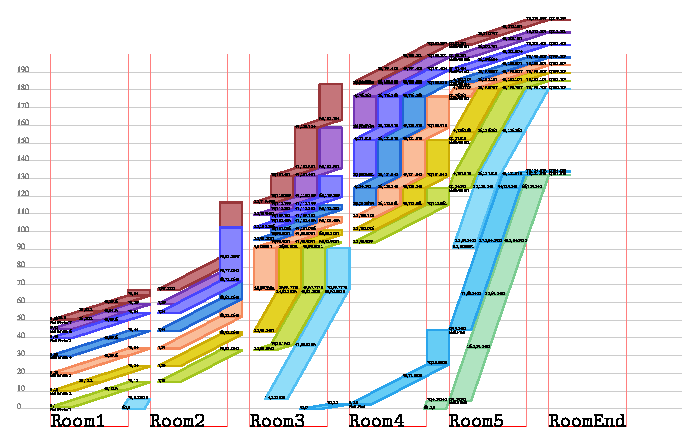
\includegraphics[angle=0,width=16cm]{50_figs/__Testing_Pipe_Zboxen.eps}
  \caption{``Balls'' moving through five ``rooms'': The time axis is
    vertical, labeled in seconds on the left, progressing upwards.
    Each ball's trajectory is a different colour. Their behaviour and
    starting points are variously described in the zsyntax input
    file. Black numbers along the trajectories are $(x,t)$ values.}
  \label{fig:balls}
\end{figure}

A Gawk program (which is unsophisticated, having some things like
labels hard-coded) is provided which extracts the movement of the
\zobj{zboxen} and plots the output in a Postscript file:\\
\comline{cat \_Testing\_Pipe\_Zboxen.zo | gawk -f Report\_to\_ps.awk > \_Testing\_Pipe\_Zboxen.eps }\\
The resulting plot is shown in \Figref{fig:balls}.

A script is provided which contains the
above commands and an additional line to convert to a PDF file.
It requires Ghostscript to be installed, as it uses {\tt ps2pdf}.
To run the example and produce also the output graph:\\
\comline{./01\_RunAndGraphResults.sh}

Mapping of report lines to segments of the plot is straightforward; for example
the first line beginning {\tt R: zbox ztype=Ball,2,1} in the {\tt .zo} file shown
corresponds to the first blue (
\includegraphics[angle=90,width=0.4cm]{50_figs/_Blue.eps})
trajectory segment visible inside {\tt Room3}. \zobj{Zbox} speeds and speed limits
are also readily visible.

In this simple example, progress of the entire simulation can be seen in a single plot.
In particular, it is to be noticed that within a \emph{Pipe}-type \zobj{zbox},
passing is not allowed, whereas in {\tt Room2} which is a \emph{Span}-type
\zobj{zbox}, overlapping trajectories are apparent.
All ball \zobj{zboxen} eventually make their way to the \emph{Sink} \zobj{zbox} {\tt RoomEnd} and quit the system.

\begin{figure}[ht]
  \centering
  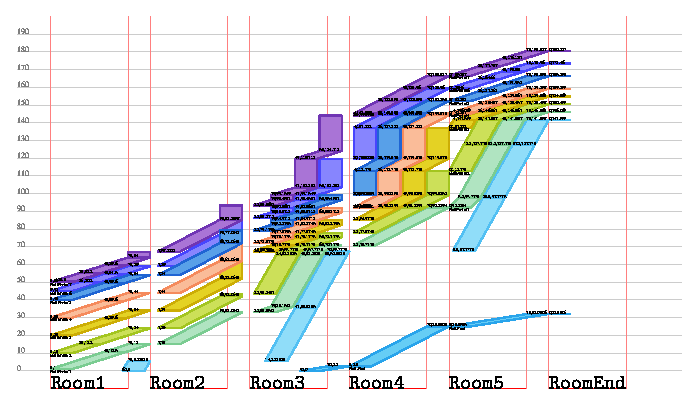
\includegraphics[angle=0,width=16cm]{50_figs/__Testing_Pipe_Zboxen2.eps}
  \caption{``Balls'' moving through five rooms: The impediment {\tt Ball.Stuck} has been removed from the system.}
  \label{fig:balls2}
\end{figure}
Commenting of the line describing {\tt Ball.Stuck}
\begin{lstlisting}[mathescape]
  # [zbox Ball.Stuck A=Ball n=1  z=<Room4>  P=<RoomTour1> i_P=3 x=67.5 v=0.55]        
\end{lstlisting}
and re-running the model, the new plot shown in \Figref{fig:balls2} is obtained.
It can be seen that without the impediment that {\tt Ball.Stuck} (
\includegraphics[angle=90,width=0.4cm]{50_figs/BallStuckColour.eps})
represented, the system of rooms behaves differently.
